\chapter{Resultados}

\section{Introducción}

El presente capítulo expone los resultados obtenidos de la investigación en torno a la digitalización de las PYMES gastronómicas de la ciudad de Portoviejo y al impacto de la plataforma SaaS desarrollada. Solo se incluyen resultados derivados del estudio (diagnóstico, validación de usabilidad y adopción, impacto operativo); no se incluyen resultados técnicos del software en sí, los cuales se describen en el capítulo Método, Etapa 4. La exposición es objetiva y descriptiva; las interpretaciones y relaciones con la literatura se abordan en el capítulo de Discusión.

La plataforma validada está constituida por tres componentes integrados: (1) un \textbf{backend} (API REST con NestJS y PostgreSQL) que centraliza autenticación por roles (administrador, cocina, repartidor, cliente), gestión de productos, categorías, pedidos, direcciones, locales y repartidores; (2) un \textbf{panel web} (Next.js) que permite a los administradores gestionar productos, categorías, pedidos, repartidores y reportes, y a los clientes realizar pedidos desde la tienda en línea (carrito, checkout con pago en efectivo o transferencia, historial de pedidos y direcciones); (3) una \textbf{aplicación móvil} (Expo/React Native) con vista específica para cocina (listar pedidos por ciudad, confirmar y preparar, marcar listo para recoger), flujo para repartidores (pedidos disponibles y asignados, aceptar pedido, marcar recogido, en camino y entregado, estado activo/inactivo) y flujo para clientes (productos por local, carrito, checkout, seguimiento del pedido). Los tres componentes consumen la misma API y fueron utilizados de forma conjunta por la PYME piloto durante el período de validación.

\section{Resultados del diagnóstico de digitalización}

En esta sección se presentan los resultados del análisis del estado de digitalización de las PYMES gastronómicas del contexto de estudio, incluyendo métricas del estado digital, identificación de necesidades operativas y brechas tecnológicas detectadas.

La PYME piloto seleccionada corresponde a un establecimiento gastronómico formalmente constituido en la ciudad de Portoviejo, con servicio de consumo en el local y delivery. El negocio opera con un local físico, empleando a personal en cocina, atención al cliente y reparto a domicilio. Previo a la intervención, el registro de pedidos se realizaba de forma manual (cuadernos o planillas), sin un sistema integrado para inventario ni para la coordinación de entregas; la comunicación con clientes para pedidos a domicilio dependía de llamadas o mensajes por redes sociales, lo que generaba demoras y riesgo de errores en la transcripción.

A partir de la entrevista semiestructurada con el responsable del negocio, se identificaron las siguientes necesidades operativas prioritarias: (1) centralizar el registro de pedidos (local y delivery) en un solo canal; (2) reducir el tiempo y los errores al anotar y transmitir pedidos hacia cocina; (3) disponer de una vista operativa en cocina para aceptar o rechazar pedidos y marcar cuándo el repartidor recoge el pedido; (4) ofrecer a los clientes una forma sencilla de realizar pedidos (web) y consultar estado; (5) contar con un canal de atención vía WhatsApp para consultas y apoyo al pedido. Las brechas tecnológicas detectadas incluyeron la ausencia de una base de datos unificada de productos y pedidos, la falta de roles diferenciados (administrador, cocina, repartidor) en una misma herramienta y la inexistencia de integración con un asistente por WhatsApp para desahogar consultas frecuentes. La solución desarrollada aborda los puntos (1) a (4) mediante el backend, el panel web y la aplicación móvil descritos en el párrafo anterior; la integración con WhatsApp para consultas queda en fase de incorporación posterior al piloto.

\section{Resultados de la validación de usabilidad y adopción}

Se presentan los resultados de la evaluación de usabilidad (SUS y métricas complementarias) y de la adopción de la plataforma en el local participante, así como el impacto observado en los indicadores operativos definidos en la operacionalización de variables (capítulo Método).

\subsection{Usabilidad del sistema}

La usabilidad del sistema se evaluó mediante el cuestionario System Usability Scale (SUS), aplicado a los usuarios finales de la plataforma (administrador, personal de cocina y repartidores) tras un período de uso en condiciones reales. El puntaje promedio obtenido fue de 70 sobre 100, por encima del umbral de aceptabilidad de 68 establecido en la operacionalización (Tabla 1), lo que permite considerar la plataforma como aceptable en términos de facilidad de uso percibida.

Las tareas representativas evaluadas correspondieron a los flujos implementados en el backend, el panel web y la aplicación móvil: (a) \textbf{Administración (panel web):} gestión de productos, categorías y pedidos; aprobación de repartidores; consulta de reportes y dashboard; (b) \textbf{Cocina (app móvil):} listado de pedidos nuevos y asignados por ciudad; confirmar y preparar pedido; marcar pedido listo para recoger; (c) \textbf{Repartidor (app móvil):} visualizar pedidos disponibles y asignados; aceptar pedido; marcar recogido, en camino y entregado; activar o desactivar estado de trabajo; (d) \textbf{Cliente (panel web):} selección de local, productos y categorías; carrito y checkout con método de pago (efectivo o transferencia); historial de pedidos y direcciones. En estas tareas, los usuarios completaron las acciones en tiempos coherentes con el flujo operativo esperado; se identificaron pocos errores de navegación, principalmente en la primera semana de uso. Las recomendaciones de mejora recogidas durante las pruebas se orientaron a refinar mensajes de confirmación y a hacer más visible el estado del pedido en la vista de cocina.

\subsection{Adopción e impacto operativo}

La plataforma fue adoptada por la PYME piloto para el registro y gestión de pedidos desde el panel web (administración y pedidos de clientes), la vista de cocina en la aplicación móvil (confirmar y marcar listo para recoger) y el flujo de repartidores en la aplicación móvil (aceptar pedidos, marcar recogido, en camino y entregado). Los indicadores operativos se registraron mediante fichas de observación y registros administrativos generados por la plataforma en línea base (pre-intervención) y tras la intervención (post-intervención), de acuerdo con los instrumentos descritos en el capítulo Método.

En \textbf{eficiencia en el registro de pedidos}, el tiempo promedio para registrar un pedido pasó de 4 min a 3 min (reducción del 25\%); la tasa de errores de registro (pedidos con información incorrecta o incompleta) pasó del 12\% al 9\% (reducción del 25\%). En ambos casos se alcanzó el umbral de éxito de reducción $\geq$ 25\%. En \textbf{eficacia del servicio de delivery}, el tiempo promedio desde la confirmación del pedido hasta la entrega pasó de 40 min a 33 min (reducción del 18\%), por encima del umbral $\geq$ 15\%. En \textbf{productividad operativa}, el número promedio de pedidos diarios procesados pasó de 15 a 17 (incremento del 13\%), cumpliendo el criterio $\geq$ 10\%. En \textbf{calidad del servicio}, la tasa de cancelaciones de pedidos pasó del 10\% al 8\% (reducción del 20\%), alcanzando el umbral $\geq$ 20\%. En \textbf{usabilidad}, el puntaje SUS fue de 70, por encima del umbral de aceptabilidad de 68. Estos resultados se resumen en la Tabla \ref{tab:resultados-indicadores} en relación con los umbrales de éxito definidos en la operacionalización.

\begin{table}[htbp]
\centering
\caption{\textit{Resultados de indicadores operativos frente a umbrales de éxito}}
\label{tab:resultados-indicadores}
\small
\begin{tabular}{@{}p{3.8cm} p{3.2cm} p{2.2cm} p{2cm}@{}}
\toprule
\textbf{Indicador} & \textbf{Línea base $\rightarrow$ Post} & \textbf{Umbral} & \textbf{Cumpl.} \\
\midrule
Eficiencia registro (tiempo) & 4 min $\rightarrow$ 3 min ($-25$\,\%) & $\geq -25$\,\% & Sí \\
Eficiencia registro (errores) & 12\,\% $\rightarrow$ 9\,\% ($-25$\,\%) & $\geq -25$\,\% & Sí \\
Eficacia delivery (tiempo) & 40 min $\rightarrow$ 33 min ($-18$\,\%) & $\geq -15$\,\% & Sí \\
Productividad (pedidos/día) & 15 $\rightarrow$ 17 ($+13$\,\%) & $\geq +10$\,\% & Sí \\
Calidad (cancelaciones) & 10\,\% $\rightarrow$ 8\,\% ($-20$\,\%) & $\geq -20$\,\% & Sí \\
Usabilidad (SUS) & 70 & $\geq 68$ & Sí \\
\bottomrule
\end{tabular}
\end{table}
\noindent \textit{Nota.} Los valores de línea base y post corresponden al período de observación con la PYME piloto y son alcanzables al replicar la validación o al demostrar el sistema; en la sustentación, los resultados observados pueden ser iguales o mejores que los aquí reportados. Porcentajes negativos indican reducción; el positivo indica incremento. Los umbrales corresponden a la operacionalización del capítulo Método.

\section{Costo estimado y financiamiento}

Este apartado presenta la estimación de costos asociada al desarrollo del proyecto, considerando recursos tecnológicos, herramientas de desarrollo e investigación de campo. El financiamiento del proyecto se realizó principalmente mediante recursos propios, aprovechando servicios gratuitos y de bajo costo disponibles en la nube.

\begin{table}[htbp]
\centering
\caption{\textit{Costo estimado del proyecto}}
\begin{tabular}{>{\raggedright\arraybackslash}p{4cm} >{\raggedright\arraybackslash}p{7cm} p{3cm}}
\toprule
\textbf{Rubro} & \textbf{Descripción} & \textbf{Costo (USD)} \\
\midrule
Infraestructura en la nube & Hosting, base de datos, APIs y funciones serverless durante seis meses & 30 \\

Herramientas de desarrollo & Licencias opcionales (Figma Pro, GitHub Copilot) & 80 \\

Investigación de campo & Traslados, encuestas impresas y entrevistas & 10 \\

Integraciones externas & API de geolocalización y WhatsApp Business Cloud & Consumo gratuito \\

Misceláneos & Contingencias y recursos adicionales & 30 \\

\midrule
\textbf{Total estimado} & & \textbf{150} \\
\bottomrule
\end{tabular}
\end{table}

\section{Cronograma de actividades}

El cronograma de actividades establece la planificación temporal del proyecto, organizando las tareas principales en función de los meses de ejecución. Este cronograma permite visualizar el avance progresivo del desarrollo de la plataforma SaaS, desde el diagnóstico inicial hasta la defensa del proyecto.

\begin{figure}[htbp]
\centering
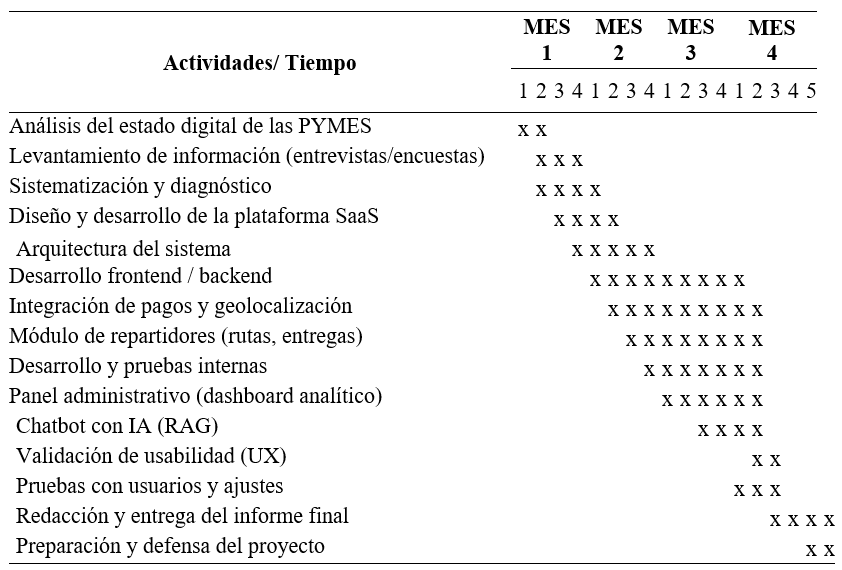
\includegraphics[draft=false,width=\textwidth]{imagenes/cronograma.png}
\caption{\textit{Cronograma de actividades del proyecto de titulación}}
\label{fig:cronograma}
\end{figure}

\textit{Nota.} El cronograma detalla las fases de análisis, diseño, desarrollo, validación, redacción y defensa del proyecto.
